\chapter{NAT}

\section{What is NAT?}

NAT provides the translation of private addresses to public addresses. Its primary use is to conserve public IPv4 addresses. A NAT router typically operates at the border of a stub network\footnote{A stub network is a network that has a single connection to its neighboring network -- one way in and one way out of the network.} (Figure \ref{NATborder}). Table \ref{ProsAndCons} shows the advantages and disadvantages of NAT.\\

\begin{figure}[hbtp]
\caption{NAT border}\label{NATborder}
\centering
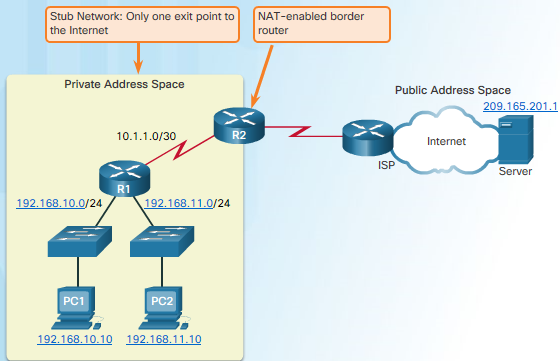
\includegraphics[ width=0.7\textwidth ]{pictures/NATborder.PNG}
\end{figure}

\begin{table}[hbtp]
\centering\caption{Pros and Cons of NAT}\label{ProsAndCons}
\begin{tabular}{ p{7cm} p{7cm} }
\toprule
\head{Advantages} & \head{Disadvantages} \\

Conserves the legally registered addressing scheme by allowing the privatization of intranets &
End-to-end functionality is degraded\footnote{NAT increases forwarding delays because the translation of each IPv4 address within the packet headers takes time.} \\

Increases the flexibility of connections to the public network &
End-to-end IP traceability is lost \\

Provides consistency for internal network addressing schemes\footnote{NAT allows the existing private IPv4 address scheme to remain while allowing for easy change to a new public addressing scheme. This means an organization could change ISPs and not need to change any of its inside clients.} & 
Tunneling becomes more complicated \\
\bottomrule
\end{tabular}
\end{table}

In NAT terminology, the inside network is the set of networks that is subject to translation. The outside network refers to all other networks. NAT includes four types of addresses:

\begin{figure}[hbtp]
\caption{Types of NAT addresses}
\centering
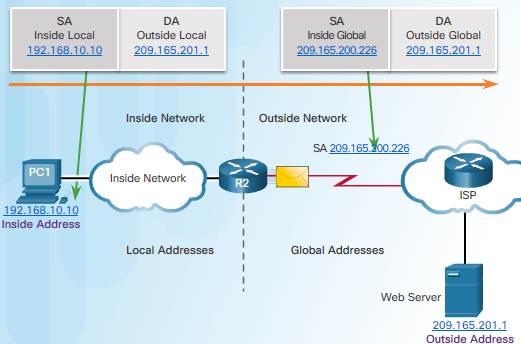
\includegraphics[ width=0.7\textwidth ]{pictures/NATterm.PNG}
\end{figure}


\begin{itemize}
\item \textbf{Inside address:} The address of the device that NAT is translating.
\item \textbf{Outside address:} The address of the destination device.
\item \textbf{Local address:} A local address is any address that appears on the inside portion of the network.
\item \textbf{Global address:} A global address is any address that appears on the outside portion of the network.
\end{itemize}

There are three types of NAT translation: static NAT, dynamic NAT, PAT (Port address translation).

\section{Operation}

In Figure \ref{NAToperation}, PC1 with private address 192.168.10.10 wants to communicate with an outside web server with public address 209.165.201.1.

\begin{figure}[hbtp]
\caption{NAT in action}\label{NAToperation}
\centering
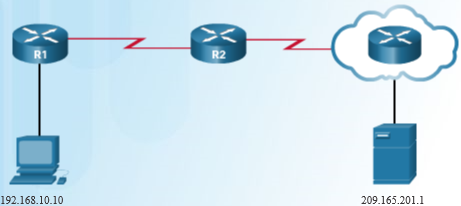
\includegraphics[ width=0.6\textwidth ]{pictures/NAToperation.PNG}
\end{figure}

When the packet arrives at R2 (NAT-enabled router), R2 reads the source IPv4 address of the packet to determine if the packet matches the criteria specified for translation. In this case, the source IPv4 address does match the criteria and is translated from 192.168.10.10 (inside local address) to 209.165.200.226 (inside global address). R2 adds this mapping of the local to global address to the NAT table. R2 sends the packet with the translated source address toward the destination.\\

The web server responds with a packet addressed to the inside global address of PC1 (209.165.200.226). R2 receives the packet with destination address 209.165.200.226. R2 checks the NAT table and finds an entry for this mapping. R2 uses this information and translates the inside global address (209.165.200.226) to the inside local address (192.168.10.10), and the packet is forwarded toward PC1.

\section{Static NAT}

Static NAT is \textbf{one-to-one} address mapping between local and global addresses. Static NAT is particularly useful for servers or devices that must have a consistent address. There are three basic steps when configuring static NAT translations:

\begin{enumerate}
\item Create a mapping between the inside local address and the inside global addresses using the \verb|ip nat inside | \verb|source static <local-ip> <global-ip>| in global configuration.

\item The interfaces participating in the translation are configured as inside or outside relative to NAT. Inside interfaces are configured with the \verb|ip nat inside| interface configuration command, whereas the outside interface is configured with the \verb|ip nat outside| interface configuration command.

\item Verify NAT configuration using \verb|show ip nat translations| or \verb|show ip nat statistics|.
\end{enumerate}

\begin{verbatim}
R2(config)# ip nat inside source static 192.168.10.254 209.165.201.5
R2(config)#
R2(config)# interface Serial0/0/0
R2(config-if)# ip nat inside
R2(config-if)# interface Serial0/1/0
R2(config-if)# ip nat outside
R2(config-if)# end
\end{verbatim}

\section{Dynamic NAT}

Dynamic NAT is \textbf{many-to-many} address mapping between local and global addresses. If there are 100 inside local addresses and 10 inside global addresses, at any given time only 10 of the 100 inside local addresses can be translated. Dynamic NAT uses a pool of public addresses and assigns them on a first-come, firstserved basis. There are six steps when configuring dynamic NAT translations:

\begin{enumerate}
\item Define the pool of addresses to be used for translation. The pool is assigned a name to identify it. Use \verb|ip nat pool | \verb|<pool-name> <start-ip> <end-ip>| \verb|netmask <netmask>|.

\item Configure a standard ACL

\item Bind the ACL to the pool. Use the \verb|ip nat inside | \verb|source list | \verb|<ACL-name>| \verb|pool| \verb|<pool-name>| global configuration.

\item The interfaces participating in the translation are configured as inside or outside relative to NAT. Inside interfaces are configured with the \verb|ip nat inside| interface configuration command, whereas the outside interface is configured with the \verb|ip nat outside| interface configuration command.

\item Verify NAT configuration using \verb|show ip nat translations| or \verb|show ip nat statistics|.
\end{enumerate}

\begin{verbatim}
R2(config)# ip nat pool NAT-POOL1 209.165.200.226 209.165.200.240 netmask 255.255.255.224
R2(config)#
R2(config)# access-list 1 permit 192.168.0.0 0.0.255.255
R2(config)#
R2(config)# ip nat inside source list 1 pool NAT-POOL1
R2(config)#
R2(config)# interface Serial0/0/0
R2(config-if)# ip nat inside
R2(config-if)# exit
R2(config)#
R2(config)# interface Serial0/1/0
R2(config-if)# ip nat outside
R2(config-if)#
\end{verbatim}

\section{PAT}

PAT (also known as NAT overloading) is a \textbf{many-to-one} address mapping between local and global addresses. With PAT, multiple addresses can be mapped to one or to a few addresses because each private address is also tracked by a port number. For example, if there are 100 inside local addresses and 10 inside global addresses, PAT uses ports as an additional parameter to provide a multiplier effect, making it possible to reuse any one of the 10 inside global addresses.\\

When the NAT router receives a packet from the client, it uses its source port number to uniquely identify the specific NAT translation. PAT ensures that devices use a different TCP port number for each session with a server on the Internet. When a response comes back from the server, the source port number, which becomes the destination port number on the return trip, determines to which device the router forwards the packets. \\

\begin{figure}[hbtp]
\caption{PAT in action}\label{PAT}
\centering
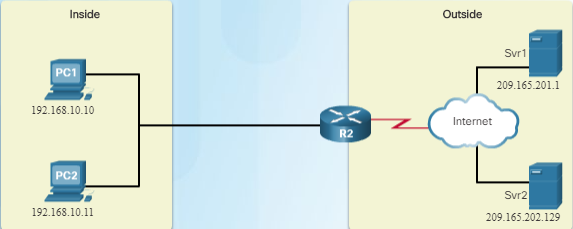
\includegraphics[ width=0.6\textwidth]{pictures/PAT.PNG}
\end{figure}

\begin{table}[hbtp]
\centering \caption{PAT table of Figure \ref{PAT} }
\begin{tabular}{ll | l}
\toprule
\head{Inside local} & \head{Inside global} & \head{Outside global} \\
\midrule
192.168.10.10:1555 & 209.165.200.226:1555 & 209.165.201.1:80 \\
192.168.10.11:1331 & 209.165.200.226:1331 & 209.165.202.129:80 \\
\bottomrule
\end{tabular}
\end{table}

In Figure \ref{PAT}, R2 uses port numbers (1331 and 1555) to identify the device from which the packet originated. In this example, the service port is 80, which is HTTP. For the source address, R2 translates the inside local address to an inside global address with the port number added. Note that, the client port numbers, 1331 and 1555, did not change at the NAT-enabled router. The destination address is the outside global IPv4 address of servers. \\

When there are no more ports available and there is more than one external address in the address pool, PAT moves to the next address to try to allocate the original source port. This process continues until there are no more available ports or external IPv4 addresses.\\

PAT also translates some protocols that do not use TCP or UDP. Each of these types of protocols is handled differently by PAT. For example, ICMPv4 query messages, echo requests, and echo replies include a Query ID. ICMPv4 uses the Query ID to identify an echo request with its corresponding echo reply. \\

There are six steps when configuring dynamic PAT translations. The six steps are identical to configuring dynamic NAT except for step 3.

\begin{enumerate}
\item Define the pool of addresses to be used for translation. The pool is assigned a name to identify it. Use \verb|ip nat pool | \verb|<pool-name> <start-ip> <end-ip>| \verb|netmask <netmask>|.

\item Configure a standard ACL

\item Bind the ACL to the pool. Use the \verb|ip nat inside | \verb|source list | \verb|<ACL-name>| \verb|pool| \verb|<pool-name>| \verb|overload| in global configuration mode. The \verb|overload| keyword is the primary difference between PAT and dynamic NAT.

\item The interfaces participating in the translation are configured as inside or outside relative to NAT. Inside interfaces are configured with the \verb|ip nat inside| interface configuration command, whereas the outside interface is configured with the \verb|ip nat outside| interface configuration command.

\item Verify NAT configuration using \verb|show ip nat translations| or \verb|show ip nat statistics|. 
\end{enumerate}

\begin{verbatim}
R2(config)# ip nat pool NAT-POOL2 209.165.200.226 209.165.200.240 netmask
255.255.255.224
R2(config)#
R2(config)# access-list 1 permit 192.168.0.0 0.0.255.255
R2(config)#
R2(config)# ip nat inside source list 1 pool NAT-POOL2 overload
R2(config)#
R2(config)# interface Serial0/0/0
R2(config-if)# ip nat inside
R2(config-if)# exit
R2(config)#
R2(config)# interface Serial0/1/0
R2(config-if)# ip nat outside
R2(config-if)#
\end{verbatim}

There are two ways to configure PAT. In the example above, we allocate more than one public IPv4 address to the inside network, and in the following, it allocates a single public IPv4 address.

\begin{enumerate}
\item Configure a standard ACL

\item Bind the ACL to the pool. Use the \verb|ip nat inside | \verb|source list | \verb|<ACL-name>| \verb|interface| \verb|<int-name>| \verb|overload| in global configuration mode. The interface mentioned in this command is the one connected to the outside network.

\item The interfaces participating in the translation are configured as inside or outside relative to NAT. Inside interfaces are configured with the \verb|ip nat inside| interface configuration command, whereas the outside interface is configured with the \verb|ip nat outside| interface configuration command.

\item Verify NAT configuration using \verb|show ip nat translations| or \verb|show ip nat statistics|. 
\end{enumerate}

\section{Port forwarding}

Port forwarding forwards traffic addressed to a specific network \emph{port} from one network node to another. In other words, in Port forwarding, NAT translate not only IP addresses but also ports that users want to access. This technique allows an external user to reach a port on a private IPv4 address (inside a LAN) from the outside, through a NAT-enabled router. A specific user usually access a single port on a server. \\

\begin{verbatim}
R2(config)# ip nat inside source static tcp 192.168.10.254 80 209.165.200.225 8080
R2(config)#
R2(config)# interface Serial0/0/0
R2(config-if)# ip nat inside
R2(config-if)# exit
R2(config)#
R2(config)# interface Serial0/1/0
R2(config-if)# ip nat outside
R2(config-if)#
\end{verbatim}

In the example, 192.168.10.254 is the inside local IPv4 address of the web server listening on port 80. Users access this internal web server using the global IPv4 address 209.165.200.225, a globally unique public IPv4 address. The global port is configured as 8080. This will be the destination port used, along with the global IPv4 address of 209.165.200.225 to access the internal web server.\\

Notice within the NAT configuration the following command parameters:

\begin{itemize}
\item local-ip = 192.168.10.254
\item local-port = 80
\item global-ip = 209.165.200.225
\item global-port = 8080
\end{itemize}